%%%%%%%%%%%%%%%%%  Debut du fichier Latex  %%%%%%%%%%%%%%%%%%%%%%%%%%%%%%
\documentclass[
    a4paper, 
    12pt, onecolumn,
    %draft
]{article}

%%% Pour un texte en francais

%%\usepackage[applemac]{inputenc}
\usepackage[T1]{fontenc}
%\usepackage[francais]{babel}
	         % encodage des lettres accentuees
\usepackage[utf8]{inputenc}          % encodage des lettres accentuees
%\usepackage{graphicx}
%%\usepackage{graphicx} \def\BIB{}
\usepackage{multicol}
\usepackage{graphicx,wrapfig,lipsum} \def\BIB{}
\usepackage[pdftex]{hyperref}
\usepackage[round]{natbib}
\usepackage{perpage} %the perpage package
\MakePerPage{footnote} %the perpage package command
\hypersetup{
    colorlinks,%
    citecolor=black,%
    filecolor=black,%
    linkcolor=black,%
    urlcolor=blue     % can put red here to visualize the links
}

\DeclareUnicodeCharacter{00A0}{ }

%%% Quelques raccourcis pour la mise en page
\newcommand{\remarque}[1]{{\small \it #1}}
\newcommand{\rubrique}{\bigskip \noindent $\bullet$ }

%\bibliographystyle{abbrvnat}
%\setcitestyle{authoryear,open={((},close={))}}

\renewcommand{\thefootnote}{\roman{footnote}}

\begin{document}

\bibpunct{[}{]}{;}{n}{,}{,}

%%%%%%%%%%%%%%%%%%%%%%%%%  PREMIERE PAGE %%%%%%%%%%%%%%%%%%%%%%%%%%%%%%
%%% DANS CETTE PAGE, ON REMPLACE LES INDICATIONS ENTRE CROCHETS [...]
%%% PAR LES INFORMATIONS DEMANDEES
%%%%%%%%%%%%%%%%%%%%%%%%%%%%%%%%%%%%%%%%%%%%%%%%%%%%%%%%%%%%%%%%%%%%%%%

 
\noindent GENCI\hfill \textsc{Demande d'Attribution de Ressources Informatiques}

\begin{center}
\Large  \bf
Scientific description of the project
\end{center}
\bigskip

\rubrique Title of the project : {\bf Numerical simulations of wind-accretion in \hspace*{4.42cm} high mass X-ray binary systems}
%Numerical simulation of Quasi-Periodic Oscillations in microquasars and comparison with observations

\rubrique  {\sc dari} number :
\hfill
%%% METTRE ICI LE RENSEIGNEMENTS DEMANDE
DARI numero c2016047469 (renouvellement de dossier)

\rubrique  Scientist in charge : 
\hfill
%%% METTRE ICI LES RENSEIGNEMENTS DEMANDES
E{\sc l mellah} Ileyk


\rubrique Laboratory :  
\hfill
%%% METTRE ICI LES RENSEIGNEMENTS DEMANDES
AstroParticule \& Cosmologie (APC) - Paris 7


%%% HEURES DEMANDEES
\rubrique  Number of hours required (mono-process {\sc cpu}) :
   %%% DECOMMENTER LES LIGNES QUI CONCERNENT LE PROJET
   %%% ET REMPLACER [1200] PAR LE RENSEIGNEMENT DEMANDE
   %%% NE METTRE QUE LES DONNEES NON-NULLES
   % \newline CCRT  BULL IA64 Platine  : \hfill  [1200] heures scalaires
   % \newline CCRT  NEC SX8R Mercure   : \hfill [1200] heures vectorielles
   % \newline CCRT  BULL X\'eon Titane : \hfill [1200] heures scalaires
   % \newline CCRT  BULL X\'eon Titane : \hfill  [1200] heures CPU/GPU
   % \newline CINES IBM SP Hera        : \hfill  [1200] heures scalaires
   %  \newline CINES SGI ICE Jade       : \hfill  300\ 000 heures scalaires
   % \newline IDRIS IBM SP Vargas      : \hfill  [1200] heures scalaires
   % \newline IDRIS IBM BG/P Babel     : \hfill  [1200] heures scalaires
   % \newline IDRIS  NEC SX8 Brodie     : \hfill  [1200] heures vectorielles
     \newline CINES BULL Occigen      : \hfill  400\ 000 scalar hours

%%% RESUME
\section{Abstract}

%%% A COMMMENTER LORS DE LA REDACTION DU PROJET
%\emph{Longueur typique de {\bf 15 lignes}, longueur maximale de {\bf 1 page}.}

%The advent of high energy observation facilities in the last decades has proven the existence of powerful mechanisms emitting photons up to gamma-rays. 
%It is now commonly admitted that the most energetic events are associated with compact objects believed to be relics of massive stars. 
%These objects are prone to the most extreme gravity fields and are likely efficient attractors of the plasma present in their vicinity. 
%The motion of plasma in the close neighborhood of compact objects is only properly described in the framework of general relativistic magnetohydrodynamic (GR- MHD). 
%The equations governing GR-MHD are so complex that the only way to solve them is trough large-scale numerical simulations. 
%The topic of the present demand,  $200\ 000$ h CPU on the parallel CINES computer \lq Jade\rq\ , 
%is to sustain a computational effort dedicated to GR-(M)HD simulations of accretion flows near compact objects and to link them to synthetic observations of the 
%associated violent events.

\indent \indent Our group is asking for 400 000 h cpu on the parallel CINES computer Occigen so as to pursue the investigations we have undertaken this summer on accretion in X-ray binaries. After having characterized the steady-state Bondi-Hoyle flow (aka planar wind accretion) on to a compact object, from the accretion radius to the vicinity of the compact body (typically 10,000 smaller), we can now investigate further the two subsequent questions that our results brought up. \\
\indent Indeed, the numerical simulations we ran on the Occigen nodes not only revealed the quantitative properties of the steady-state Bondi-Hoyle flow (such as the mass accretion rate) but also the qualitative ones. In particular, it turned out that a topological property concerning the sonic surface was confirmed by those simulations, a property first derived by \citep{Foglizzo1996}, which drove us into paying more attention to an entailed possibility : the formation of a resonant cavity between the shock front of the flow and the underneath sonic surface. Starting from the previous results, we designed a less diffusive mesh and used a less diffusive numerical solver in order to monitor the growth, from the steady-state, of the instability which could form, the so-called "advective-acoustic" instability \citep{Foglizzo2009}. \\
\indent In addition of the first characterization of this new instability, we started to relax the axisymmetric assumption we enforced in our 2.5D numerical setup. In a binary system, the orbital effects such as the Coriolis force no longer enable us to consider the incoming flow as planar. Considering simple cooling and heating functions, we want to assess the possibility to form a disc in a wind accretion system, a question much less explored than the formation of an accretion disc by Roche lobe overflow : and if a disc forms, how different is it from the classical $\alpha$-disc modeled by \cite{Shakura1973}? The three-dimensional characterization of such flows is a crucial prerequisite to better appreciate both the expected X-ray time variabilities and the initial conditions from which close-in accretion discs ought to be modeled.\\

\section{General presentation}

%%% A COMMMENTER LORS DE LA REDACTION DU PROJET
%\emph{Longueur typique {\bf 2 pages}, longueur maximale de {\bf 4 pages}. Si le projet se d\'ecompose en sous-projets, {\bf 2 pages additionnelles maximum par sous-projets}.}
%\vskip 0.2cm  
%\emph{Cette partie doit montrer l'int\'er\^et scientifique du projet. Le canevas suivant est propos\'e : 
%pr\'eciser les objectifs,
%situer les travaux de l'\'equipe sur le th\`eme de recherche propos\'e tant vis \`a vis du travail d\'ej\`a  
%effectu\'e par l'\'equipe (r\'esultats acquis sur le sujet), que vis \`a  vis d'autres travaux sur un plan national
%et international,
%donner une liste de publications de l'\'equipe dans le domaine dans la section \ref{Sec:Biblio}. On peut joindre au dossier tous les documents (en format pdf) annexes jug\'es utiles.}

\indent \indent The number of wind accreting systems has dramatically increased as the recent space missions stretched the limits of the high energy part of the light spectrum \citep{Liu2006,Walter15}. Once believed to be rare \citep{Illarionov1975}, those X-ray luminous objects where a compact object orbits an evolved {\sc O}/{\sc B} star (SgXB for Supergiant X-ray Binaries) did not fit well in the previously sketched categories. The characterization of the companion star is usually a challenge in itself because of the high obscuration occurring in those systems but the recent inflation of the number of extragalactic high mass X-ray binaries partly lifted this difficulty. Still, the main information we get from those objects comes from the X-ray emission to which they owe their name.\\
\begin{table}[h]
\centering
\begin{tabular}{||c|c|c||}
\hline\hline
Names & Status & Laboratory \\\hline
EL MELLAH Ileyk & Doctorant & APC\\ \hline 
CASSE Fabien & Ma\^itre de conf\'erence & APC \\ \hline
DODU Fabrice & Ing\'enieur de recherche &APC \\ \hline
\hline\hline
\end{tabular}
\caption{Members of the collaboration}
\end{table}

\indent This hard radiation, first discovered in 1962 \citep{Giacconi1962}, brought up so many questions which remain puzzling when one attempts to explain the different "families" of behaviours observed - if that an agreement is found on the very classification. Those complex systems have been dissected (the launching of the stellar wind, its orbital trajectory, the shocks it can form, its subsequent accretion onto the compact objects, etc) but in order to go beyond toy-models, which only set the asymptotic separated behaviours, one needs to tackle the entire dynamics of the stellar material, from the clumpy wind scale down to the close vicinity of the compact object (being, in our study, around a hundred gravitational radii for a black hole or the magnetosphere radius of a neutron star). For instance, being able to corroborate the identity of the compact object deduced from orbital considerations would bring more scientific weight to the current observational constraints on the equation of state of matter in neutron stars. So as to achieve such assessment, one must first wonder how the orbital parameters (the orbital period, the mass of the compact object, the mass ratio and possibly, the eccentricity) and the properties of the stellar companion (wind velocity, ejection mass rate, clumpiness) prescribe the compact object environment to disentangle the contingent from the essential causes.\\
\subsubsection*{A robust setup which revealed a previously unseen instability}
\begin{wrapfigure}{l}{6cm}
%\caption{A wrapped figure going nicely inside the text.}
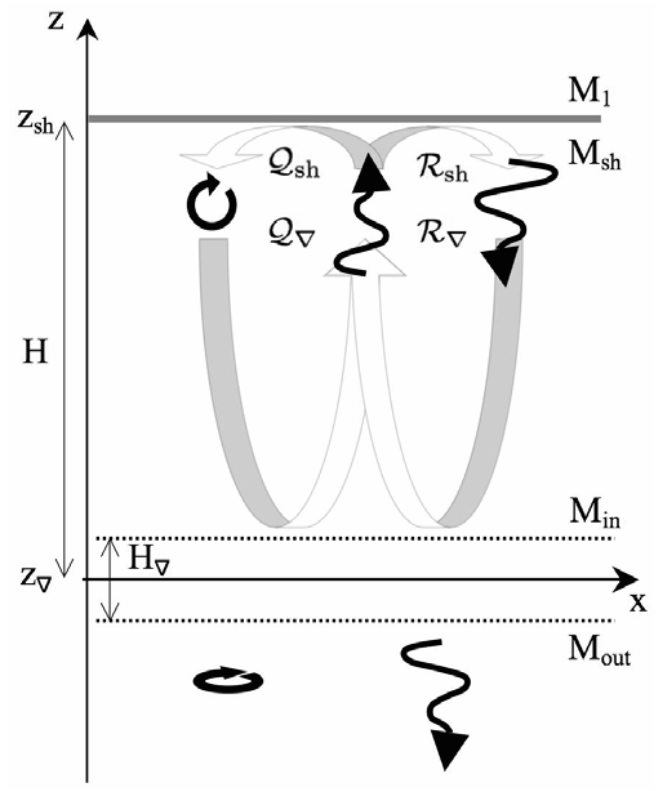
\includegraphics[height=7cm, width=6cm]{ad_ac_cylce_sketch}
\caption{Sketch of the advective-acoustic cycle between the shock at $z_{sh}$ and a subsonic zone of strong gradients, on the upper side of the sonic surface at $z_{\nabla}$. See \cite{Foglizzo2009} for more details.}
\label{fig:cycle}
\end{wrapfigure} 
\indent \indent It is precisely what we undertook thanks to the first hoursCPU we were granted in July 2015. We tested the robustness of our 2.5D axisymmetric setup and managed to witness previously unseen qualitative and quantitative properties of the flow (its structure, the mass accretion rate, the topology of the sonic surface - see "rapport d'activit\'e"). Those findings have been described in more details in a paper we published in October 2015 \citep{ElMellah2015} and brought up an unexpected question concerning a recently analytically discovered instability, the "advective-acoustic" one \citep{Foglizzo2009}. Indeed, our simulations suggested that the flow had converged towards a steady-state we characterized ; although the results were resolution independent, there was a risk than the numerical solver we were using (the total variation diminishing Lax Friedrichs), known for being a diffusive one, could damp any resonance able to make the instability grow at a sensible level. Then, we took the most of the CINES facilities to run very high resolution simulations with a much less diffusive solver (one relying on a monotonic upstream-centered scheme), starting from an interpolated version of the steady-state we had obtained. As a result, the part of the region between the shock front and the sonic surface, ahead of the accretor, turned out to be a resonant cavity where entropic perturbations are advected by the inflow and excite, as they get closer from the sonic surface, acoustic waves which travel back upstream, towards the front shock. The shock is then moving back and forth as the acoustic waves reach it, exciting new entropic perturbations. The advective-acoustic cycle is illustrated on Figure\,\ref{fig:cycle}, from \citep{Foglizzo2009}.\\
\begin{figure}
\begin{center}
%\caption{A wrapped figure going nicely inside the text.}
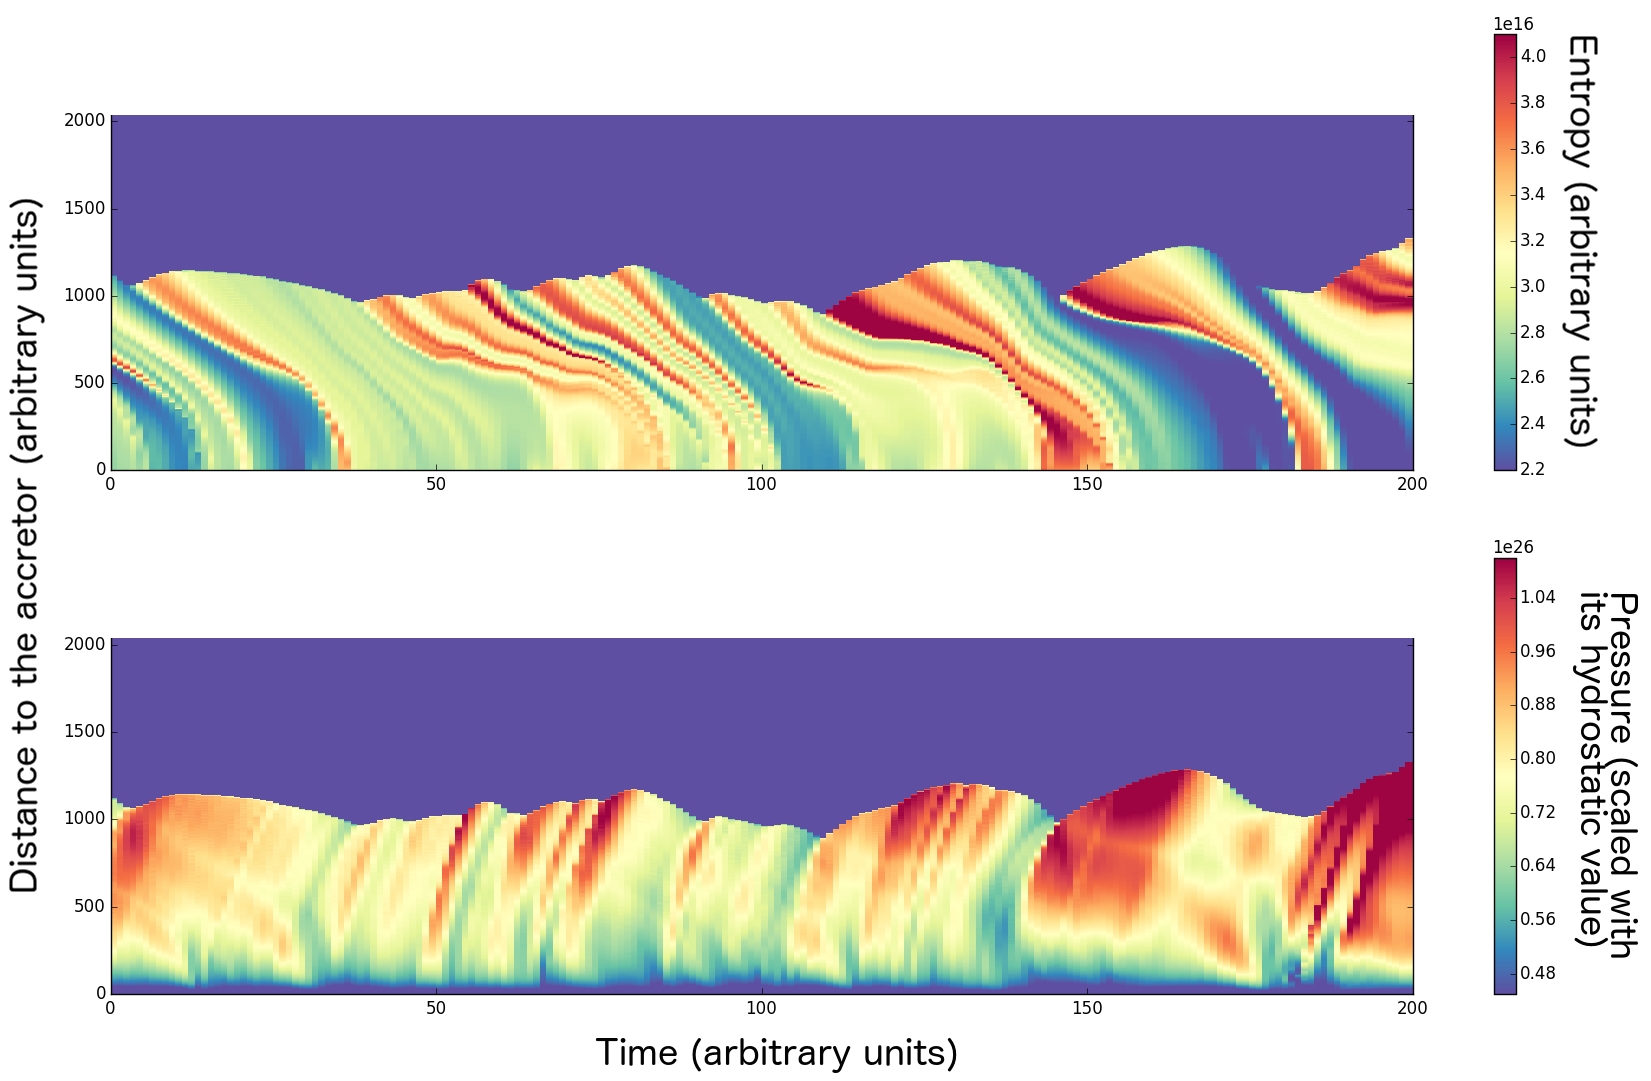
\includegraphics[width=12cm]{waves.png}
\caption{Colormaps of the entropy (upper panel) and of the deviation compared to hydrostatic equilibrium pressure (lower panel) as a function of time (horizontal axis) and of distance towards the accretor (vertical axis) which lies at the bottom. The waterline at the top stands for the position of the shock front, which is pushed upstream each time it is reached by a pressure wave. The flow is supersonic on the upper side of this border and subsonic just below. The very bottom blue part in the lower panel corresponds to the inner supersonic region, below the sonic surface, where the acoustic waves can no longer travel upstream.}
\label{fig:waves}
\end{center}
\end{figure} 
\indent If the growth of this instability has been thoroughly characterized the last decade, its saturation level remains totally unknown. Could this instability account for some of the many time variabilities observed in systems where a compact object undergoes wind accretion? Beyond the case of the X-ray binaries lie the runaway compact bodies which have been kicked at supersonic velocities with respect to the interstellar medium because of an assymetric explosion or in a close encounter - see eg \cite{Sperhake2011}. Several neutron stars have been witnessed in this regime (eg IGR J11014-6103) and the question of shock cone vibrations is under investigation \citep{Lora-Clavijo2013}. It has also been suggested that another instability, non-axisymmetric and coined as the "flip-flop instability", could be responsible for the quasi-periodic oscillations seen in some X-ray binaries \citep{Donmez2011}. If we are granted the requested hours on the Occigen BULL cluster, we intend to investigate the growth of this instability (to make sure it corresponds to the advective-acoustic one) and its saturation level. The interplay between inflowing entropic waves and outflowing acoustic ones we have glimpsed in our very first simulations is already very promising (see Figure\,\ref{fig:waves}).


\subsubsection*{Towards a comprehensive numerical setup for wind accreting XB}
\begin{wrapfigure}{l}{6cm}
%\caption{A wrapped figure going nicely inside the text.}
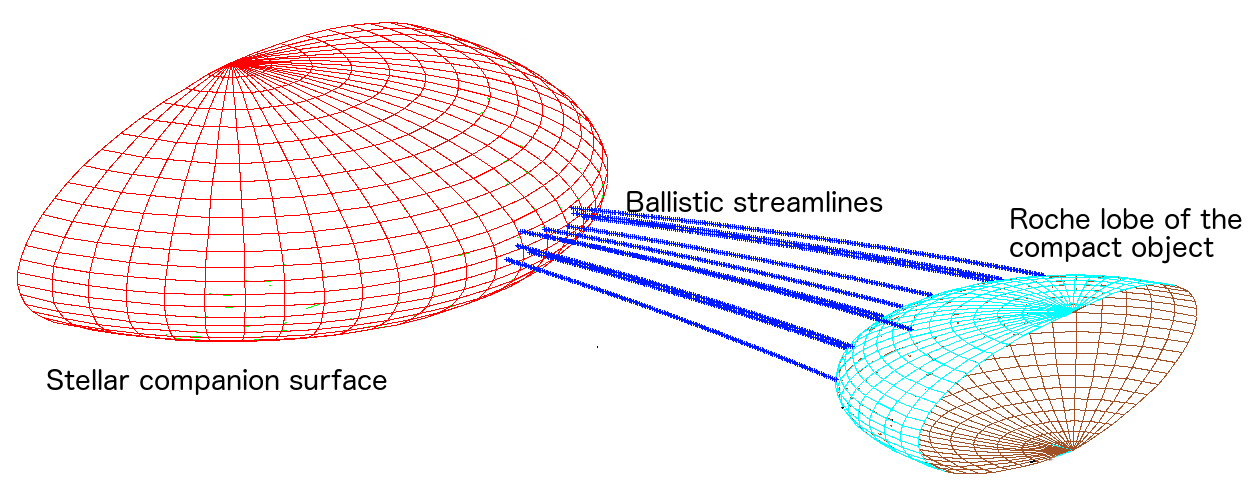
\includegraphics[height=4cm, width=6cm]{B1.png}
\caption{Sketch of some computed ballistic streamlines a supersonic wind would follow from the stellar surface (on the left) to the Roche lobe of the compact object (on the right)}
\label{fig:streamlines}
\end{wrapfigure} 
\indent \indent It has been long known that the binary systems hosting a compact object can see the stellar companion fill its Roche lobe, which results in the formation of an accretion disc as matter is gently poured through the first Lagrangian point. If this picture holds for low-mass X-ray binaries, it does not do much to account for the X-ray luminosity of high-mass X-ray binary systems where, in much cases, the stellar companion is enclosed within its Roche lobe. The mass transfer occurs either when the compact companion, on an eccentric orbit, passes by the decretion disc surrounding a rapidly rotating star (BeHMXB) or through the intense stellar wind of a supergiant stellar companion (SgXB). In the latter case, the compact body undergoes a similar kind of accretion as the one previously described except that the wind arriving is not planar ; from the stellar surface to the Roche lobe of the compact object, it has been twisted by the Coriolis force and the Roche potential.\\
\indent So as to apply the previously designed logarithmically stretched grid to this case, we decided to focus our simulations space on the compact object : it roughly fits the Roche lobe (the light blue sphere on the Figure\,\ref{fig:streamlines}.). Yet, to account for the non planar outer boundaries conditions, we wrote and used a ballistic integrator to draw the streamlines of a supersonic flow, from the stellar surface to the Roche lobe of the compact object. In addition of giving us physically motivated outer boundary conditions, this code gave us the occasion to partly disentangle the orbital parameters (the mass ratio, the mass of the compact object and the orbital period) from the ones specific to the flow (its clumpiness, its temperature, etc). As a consequence, we could assess the fraction of the outflowing stellar wind passing within the Roche lobe of the compact object, which gives us an upper limit on the mass accretion rate (related to the X-ray luminosity) and on the angular momentum accretion rate (which evaluates the odds to get a disc instead of a direct impact system), see Figure\,\ref{fig:mdot}.
\begin{figure}
\begin{center}
%\caption{A wrapped figure going nicely inside the text.}
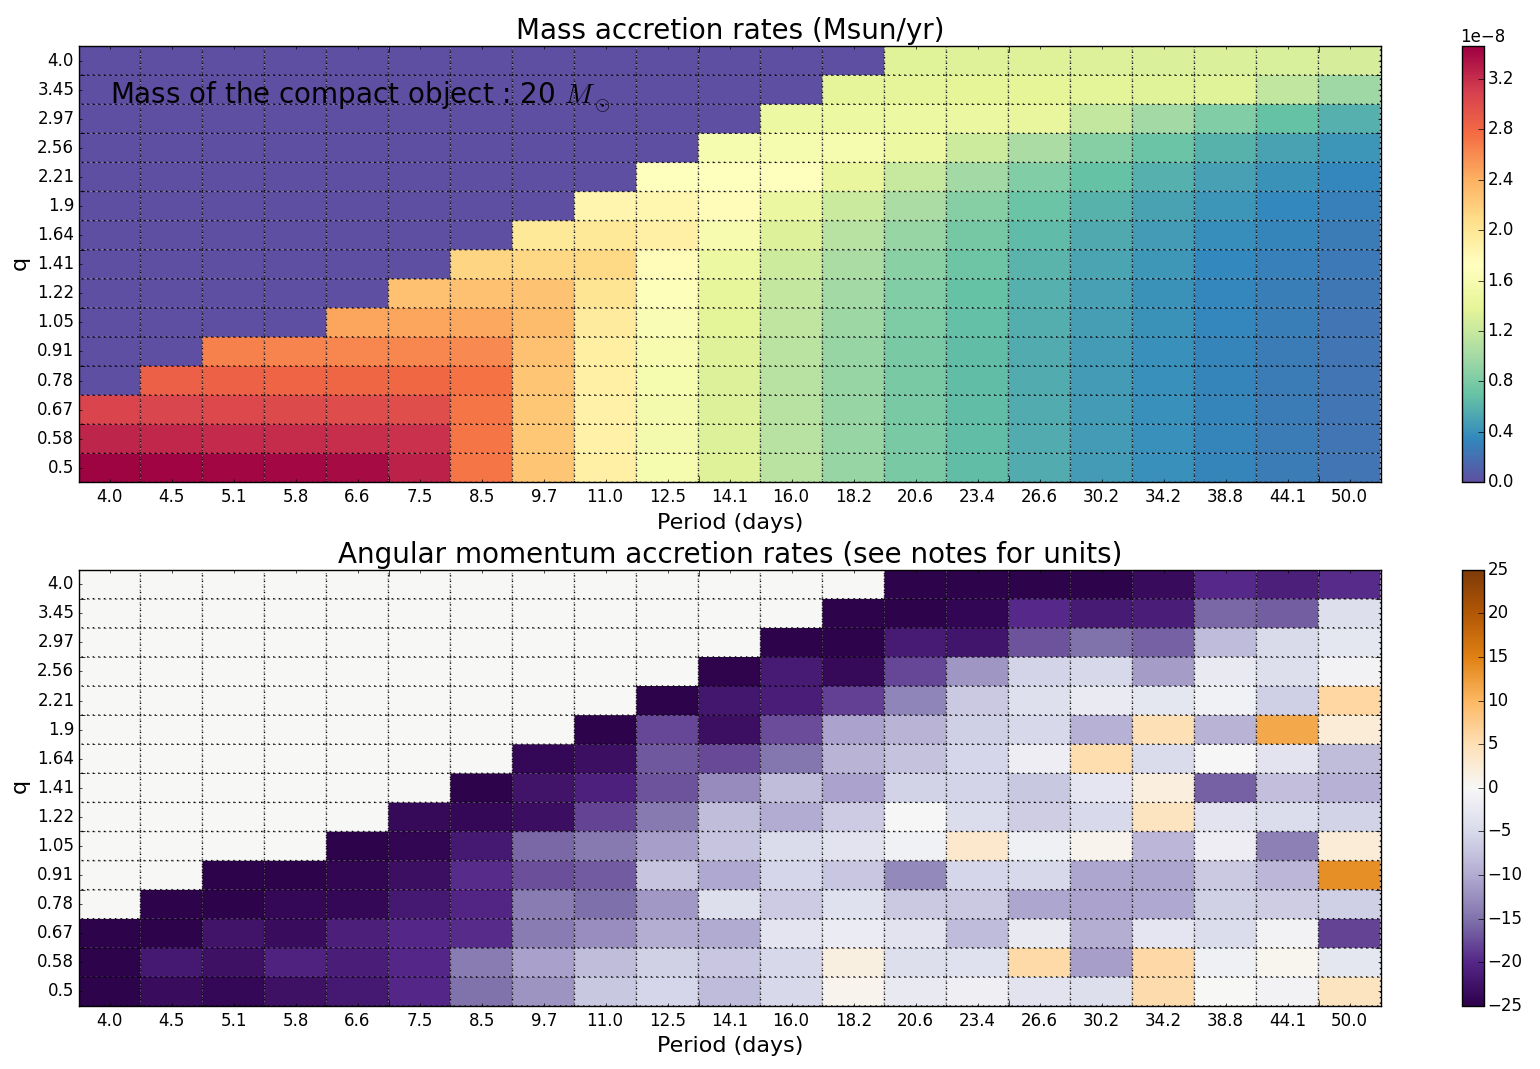
\includegraphics[height=8cm, width=13cm]{20sun_masses.png}
\caption{For a 20 solar masses compact object, colormaps of the mass and angular momentum inflowing within the Roche lobe as a function of the orbital period and of the mass ratio (given by the stellar mass divided by the mass of the compact object). The upper left corner corresponds to the Roche lobe overflow regime.}
\label{fig:mdot}
\end{center}
\end{figure} 
 The mass accretion rates converted into X-ray luminosities are typically 2 orders of magnitude higher than the observed ones, suggesting that among the inflowing gas within the compact object Roche lobe, only a fraction will actually be accreted once dissipative effects come into play. We are now able to spot the orbital configurations likely to give birth to (i) luminous X-ray wind accreting systems (the SgXB are bright and persistent sources) and to (ii) accretion discs. \\
\\
\indent Finally, it is noteworthy that our work also aims at constraining future and incoming observational mission (\href{http://www.the-athena-x-ray-observatory.eu}{{\sc athena}} \& \href{http://astro-h.isas.jaxa.jp/en/}{{\sc astro-h}} eg) : which waveband should we look after? Which time scale should we aim to characterize processes involved in the building up of an accretion disc in a wind accreting configuration? Since the mass accretion rate determines the available power convertible into X-ray luminosity, such simulations would also set lower limits for the sensibility required to probe events taking place in the very neighborhood of the compact object. The related studies, led in parallel, of the instabilities in this strong gravitational field regims (the {\sc nova}s project eg) might, one day, tell us more about the Physics at stake in those extreme environments : what kind of hitherto unseen events can take place in the wildness of a neutron star light cylinder or of a black hole ergosphere?


\section{Method}

%%% A COMMMENTER LORS DE LA REDACTION DU PROJET
%\emph{Cette partie doit \^etre suffisamment pr\'ecise et argument\'ee pour permettre au Comit\'e Th\'ematique d'appr\'ecier 
%l'ad\'equation de l'architecture
%pr\'evue (scalaire, vectorielle ou parall\`ele, GPU ...) au probl\`eme pos\'e. Il convient aussi de justifier clairement la n\'ecessit\'e de l'utilisation d'un tr\`es grand \'equipement pour le traitement informatique du projet.
%Voici une proposition de plan (\`a adapter selon le sujet) :
%Algorithme utilis\'e, adaptation \`a la plate-forme vis\'ee; Modalit\'es d'optimisation (vectorisation, optimisation superscalaire, parall\'elisation); Structure du programme; Logiciels n\'ecessaires; Langages utilis\'es; Biblioth\`eques pr\'evues; Syst\`emes de gestion de bases de donn\'ees ou syst\`emes documentaires utilis\'ees.}


\subsection{Numerical tools}

%%% A COMMMENTER LORS DE LA REDACTION DU PROJET
%\emph{Longueur typique de  {\bf 4 pages}, longueur maximale de {\bf 6 pages}.}

\subsubsection*{The \textbf{\textsc {mpi-amrvac}} code}

%\indent The code {\sc mpi-amrvac} (Message Passing Interface - Adaptative Mesh Refinement Versatile Advection Code) is an {\sc amr} code parallelized with Open{\sc mpi}. This code was created to be used in a wide variety of physical applications that can be described by a set of conservative equations, independently of their nature (fluids or dust). Among the pre-existing physics modules there are modules to see the hydrodynamical and {\sc mhd} equations in the classical or special relativity case. Several types of solver are also implemented, for example Total Variation Diminishing ({\sc tvd}) L{\sc ax}-F{\sc riedrichs} or H{\sc arten}-L{\sc ax}-V{\sc an} L{\sc eer} ({\sc hll}) solvers.\\ 
%\indent The {\sc amr} grid structure is based on the use of sub-grids (of a few tens of cells in every dimension) in a tree architecture (octree in 3D). At each iteration the code uses an internal L{\sc ohner}'s method or user-supplied criteria to determine if a sub-grid needs to be refined, left as it is, or unrefined. The tree structure replaces each refined sub-grid by a $2^D$ sub-grid of the same cell-size but with the area of each cell less by a factor $2^D$. {\bf For the present project, we will probably not use the adaptative mesh refinement but instead we designed a non-regular grid fitting the geometry of the system and enabling us to reach outer radius to inner radius ratio up to $10^5$ at a low computational cost. The grid is designed to maintain the same radial to azimuthal cell size ratio constant for any radius of the simulation (Ileyk tu pourrais montrer un exempt de grille). The smallness of the cells close to the inner boundary sets the C{\sc ourant}-F{\sc riedrichs}-L{\sc ewy} ({\sc cfl}) time step so small that several tens of millions of iterations are expected in order to describe the flow dynamics. Such computation can only be achieved using a large number of {\sc cpu} available on supercomputers.}
 \begin{figure}
\centering
 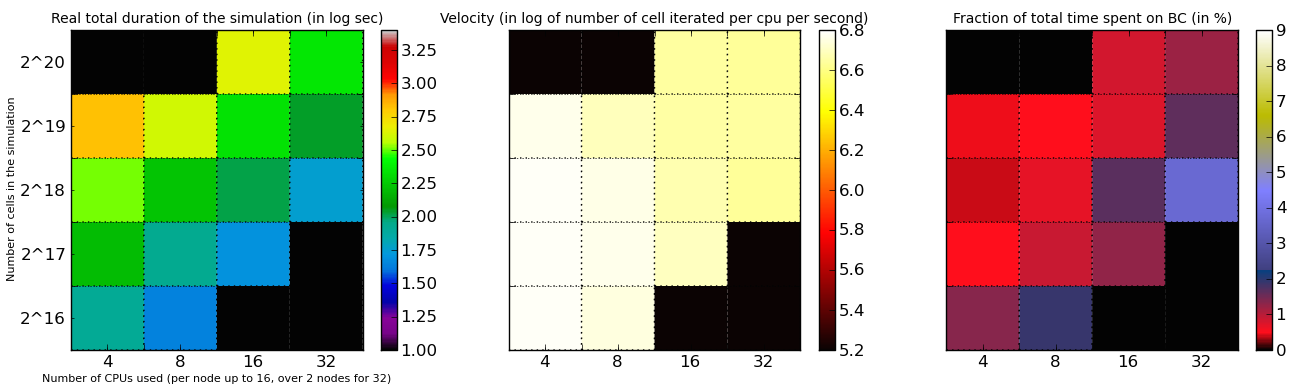
\includegraphics[width=14cm,height=5cm]{Scaling_node_14_15_unthreaded.png} 
 \caption{General scaling of the MPI-AMRVAC code performed on the Fran\c cois Arago Center ({\sc fac}e) cluster at Paris 7 Diderot} 
 \label{fig:scaling_FACe}
\end{figure}
\indent \indent The code {\sc mpi-amrvac} (Message Passing Interface - Adaptative Mesh Refinement Versatile Advection Code) is an {\sc amr} code parallelized with Open{\sc mpi}. This code was developed to solve {\sc hd} and {\sc mhd} hyperbolic conservative equations, whether in a classical or a relativistic framework. The user-defined additional source terms\footnote{Radiative cooling (in optically thick or thin regims), gravity, viscosity...} entitle to explore a wide range of physical one or two-fluids configurations. Several types of R{\sc iemann} solvers are implemented (R{\sc oe} and H{\sc arten}-L{\sc ax}-V{\sc an} L{\sc eer} ones eg), along with flux-limiter schemes as the Total Variation Diminishing ({\sc tvd}) ones.\\
\indent The {\sc amr} grid structure is based on the use of sub-grids (of a few tens of cells in every dimension) in a tree architecture (octree in 3D). At each iteration the code uses an internal L{\sc ohner}'s method or user-supplied criteria to determine if a sub-grid needs to be refined, left as it is, or unrefined. The tree structure replaces each refined sub-grid by a $2^D$ sub-grid of the same cell-size but with the area of each cell less by a factor $2^D$. For the present project, we will not use the {\sc amr} but instead, we designed a non-regular grid fitting the geometry of the system and enabling us to reach outer radius to inner radius ratio up to $10^5$ at a low computational cost. The grid is designed to maintain the same radial to azimuthal cell size ratio constant for any radius of the simulation. The smallness of the cells close to the inner boundary sets the C{\sc ourant}-F{\sc riedrichs}-L{\sc ewy} ({\sc cfl}) time step to such small values that several tens of millions of iterations are expected in order to describe the flow dynamics both at large and small scales. Such computation can only be achieved using the large number of {\sc cpu} available on supercomputers.
\newline

\subsubsection*{Parallelization and scaling}
\begin{wrapfigure}{r}{6cm}
\vspace*{-60pt}
%\caption{A wrapped figure going nicely inside the text.}
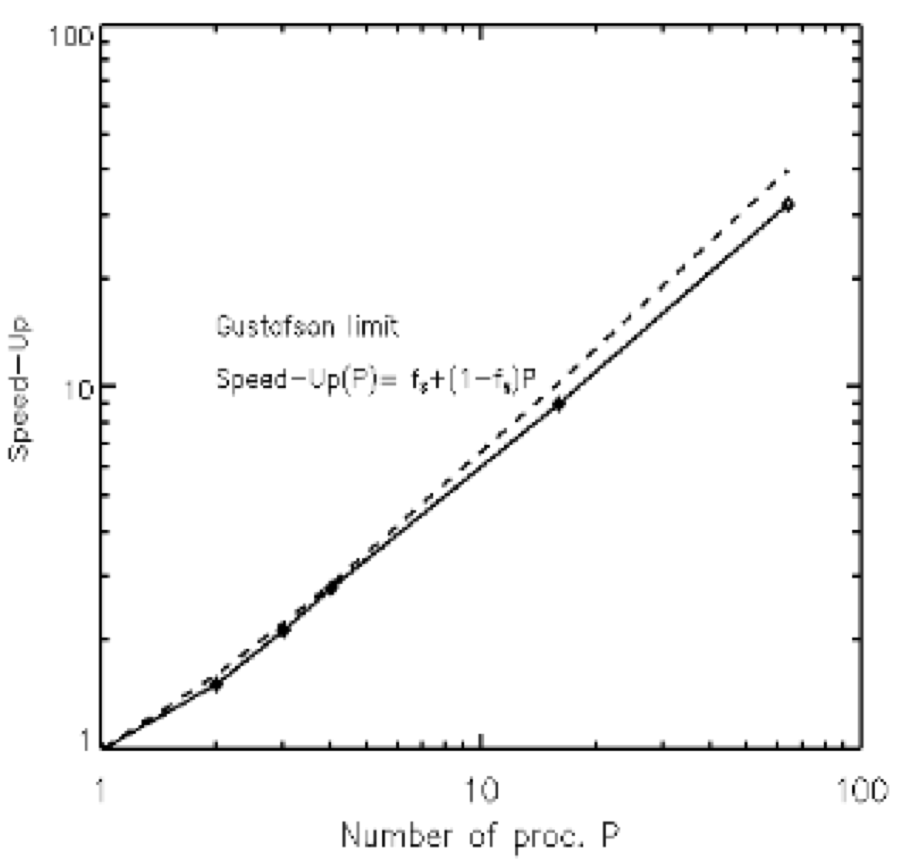
\includegraphics[height=6cm, width=6cm]{scaling_1}
\caption{Scaling of the MPI-AMRVAC code performed on the JADE super-computer}
\label{fig:scaling_JADE}
\end{wrapfigure} 
\indent \indent The parallelization relies on Open{\sc mpi} libraries and the scalability test done on \lq Jade\rq  by Zakaria M{\sc eliani} has showed an efficiency of the order of 80\% on 2000 processors (see Figure\,\ref{fig:scaling_JADE}). This value is very close to the theoretical limit when one takes into account the I/O of the code needed to write the data. Those results of the parallelization efficiency were obtained using a test case in relativistic hydrodynamics, taking into account the propagation of shocks with Lorentz factors between 100 and 1000. The main test was done in 2D with 10 levels of {\sc amr} with a refinement ratio of 2. This allowed us to locally increase the resolution of the simulation by a factor of $218$. The {\sc mpi-amrvac} code also includes two different methods to write the data allowing a better flexibility. Indeed, {\sc mpi-amrvac} can either use the method  MPI-II/IO or the method that consists of sending all the data from the slave node to the master node to minimise the number of processors taking part in the writing.

\subsection{Time justification}

\indent \indent If the logarithmically stretched grid we developed enables us to investigate this intrinsically multi-scale problem at an affordable cost, the huge time dynamics entailed precludes extended numerical simulations on local clusters as the \href{http://www.apc.univ-paris7.fr/FACe/en/cluster-arago}{{\sc fac}e} one (see Figure\,\ref{fig:scaling_FACe}). For non axissymmetric outer boundary conditions, we still require the computational ability to monitor the full 3D flow over large scale time scales, which implies hundreds of 10$^6$ iterations.\\
\indent We consider here the most demanding numerical simulations ie the full 3D one (the 2.5D ones will be launch depending on the remaining computing time available). To better assess the time needed for our 3D simulations, one can consider the following elements :
\begin{itemize}
\item in the nominal conditions of use with {\sc mpi}-{\sc amrvac}, the number of cells iterated per processor per second, $v$, is of the order of one million
\item we intend to run full 3D simulations with spatial resolutions between $176\times 32\times 128 \sim 0.7$ million cells and $256\times 64\times 256 \sim 4$ millions cells
\item to limit the communication time between {\sc cpu}s, we will use subgrids of size $16\times 16\times 16$ (not smaller) and will set the number of subgrids per {\sc cpu} to 4, which means that we can run simulations on 44 to 256 {\sc cpu}s (depending on the resolution)
\end{itemize}
The real duration of a simulation (in seconds) is then given by $N_{it}/50$, where $N_{it}$ is the number of time iterations we want to compute. Let us consider that we want to run those simulations over one orbital period. If we compare the orbital period $P$ of an X-ray binary hosting a star of mass $M_1$ and a compact object of mass $M_2$ with a semi-major axis $a$, to the numerical time step $\Delta t$ given by the gravitational one\footnote{Usually more constraining than the {\sc cfl} one in this configuration.}, we have, for a wind with a velocity at infinity of $v_{\infty}$ : 
\begin{equation}
N_{it}=\frac{P}{\Delta t}=300\cdot 10^{\frac{3}{2}n} \left(\frac{v_{\infty}}{10^3\texttt{km}\cdot\texttt{s}^{-1}}\right)^3
 \left(\frac{a}{0.1\texttt{AU}}\right) f(M_1/10M_{\odot},M_2/10M_{\odot})
\end{equation}
$f$ being given by :
\begin{equation}
f(x,y)=\sqrt{\frac{2}{y^2(x+y)}}
\end{equation}
The aspect ratio of the cells has been set to 1 here. The $n$ exponent stands for the relative size of the inner radius $r_{in}$ compare to the accretion radius $\zeta _{\textsc{hl}}$ : $r_{in}=10^{-n}\zeta _{\textsc{hl}}$. The numerical values considered here are the expected figures for a wind accreting {\sc hmxb}. Such as to approach the actual size of the accreting body, we want $n$ to be as high as possible\footnote{The higher $n$ the deeper into the gravitational potential those simulation go.} (see also Figure 1 of the rapport d'activit\'e, the vertical axis on the right). The table below is a summary of the computing cost and actual duration of those 3D simulations for different values of the $n$ exponent and with a run on 256{\sc cpu}s.
\begin{table}[h]
\centering
\begin{tabular}{|c|c|c|c|}
\hline
n & N$_{it}$ & Duration & kh$\cdot${\sc cpu} \\\hline
2 & 3$\cdot$10$^5$ & 2 hours & 0.5\\ \hline 
3 & 10$^7$ & 2 days & 12 \\ \hline
4 & 3$\cdot$10$^8$ & 70 days & 430 \\ \hline
\end{tabular}
\end{table}
If we did manage to go down to $n=4$ in the 2.5D simulations previously mentioned, it is clear that such a spatial and time dynamics will be difficult to reach in 3D but we still think we can get important results with inner boundaries given by $n=3$ where the inner boundary would be of the order of 100 times the actual Schwarzschild radius of a 10 solar masses black hole. Each simulation would require 12 kh$\cdot${\sc cpu} and we need to explore several sets of orbital parameters ($P$,$M_2$,$M_1/M_2$), 5 for instance, each with different numerical processing or with different physical parameters for the incoming wind. Such an exploration would require a very minimum of 5$\times$6$\sim$30 runs to indicate the first tendencies and direct our next studies, hence our request for 400,000 kh$\cdot${\sc cpu}. If additional hours are necessary, we intend to apply in April for the proc\'edure d'attribution compl\'ementaire.   
\cite{ElMellah2015}\cite{ElMellah2015a}\cite{Rappaport2013}\cite{Rappaport:2012wi}\cite{SanchisOjeda:2014ww}\cite{ElMellah2015b}

\newpage\section{Bibliographie}
\label{Sec:Biblio}
 
\bibliographystyle{plainnat}
\bibliography{/Users/ielm/Documents/Bibtex/My_articles}

\end{document}
%%%%%%%%%%%%%%%%%  Fin du fichier Latex  %%%%%%%%%%%%%%%%%%%%%%%%%%%%%%

